% Documento LaTeX completo (modo raw PDF 1:1) — plantilla tipo paper de lab
\documentclass[11pt,a4paper]{article}
\usepackage[margin=2.5cm]{geometry}
\usepackage{fontspec}
\usepackage{amsmath,amssymb,mathtools}
\usepackage{booktabs,siunitx}
\usepackage{graphicx}
\usepackage{tikz}
\usetikzlibrary{decorations.markings,decorations.pathmorphing,arrows.meta}
\usepackage[hidelinks]{hyperref}

\title{Fixture de estrés lablog}
\author{Suite de pruebas}
\date{\today}

\begin{document}
\maketitle

\begin{abstract}
Documento completo para validar el camino raw de Tectonic: símbolos,
matrices, tabla booktabs y un diagrama TikZ tipo Feynman.
\end{abstract}

\section{Símbolos}
\[
\alpha+\beta=\gamma,\quad
\sum_n \frac{1}{n^2}=\frac{\pi^2}{6},\quad
\hbar,\ \nabla\cdot\mathbf{J}+\partial_t\rho=0
\]

\section{Matriz}
\[
U = \begin{pmatrix}
\cos\theta & -\sin\theta \\
\sin\theta & \cos\theta
\end{pmatrix}
\in \mathrm{SO}(2)
\]

\section{Tabla}
\begin{center}
\begin{tabular}{l S}
\toprule
{Observable} & {Valor} \\
\midrule
$m_e$ & 0.511 \\
$m_\mu$ & 105.7 \\
\bottomrule
\end{tabular}
\end{center}

\section{Diagrama}
\begin{center}
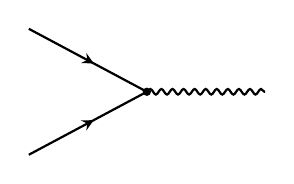
\begin{tikzpicture}[
  fermion/.style={thick, postaction={decorate},
    decoration={markings, mark=at position 0.55 with {\arrow{stealth}}}},
  photon/.style={decorate, decoration={snake, amplitude=1pt, segment length=4pt}, thick}
]
  \draw[fermion] (-1.5,0.8) -- (0,0);
  \draw[fermion] (-1.5,-0.8) -- (0,0);
  \draw[photon] (0,0) -- (1.5,0);
  \fill (0,0) circle (1.5pt);
\end{tikzpicture}
\end{center}

\end{document}
